\documentclass[12pt,letterpaper]{article}
\usepackage{graphicx,textcomp}
\usepackage{natbib}
\usepackage{setspace}
\usepackage{fullpage}
\usepackage{color}
\usepackage[reqno]{amsmath}
\usepackage{amsthm}
\usepackage{fancyvrb}
\usepackage{amssymb,enumerate}
\usepackage[all]{xy}
\usepackage{endnotes}
\usepackage{lscape}
\newtheorem{com}{Comment}
\usepackage{float}
\usepackage{hyperref}
\newtheorem{lem} {Lemma}
\newtheorem{prop}{Proposition}
\newtheorem{thm}{Theorem}
\newtheorem{defn}{Definition}
\newtheorem{cor}{Corollary}
\newtheorem{obs}{Observation}
\usepackage[compact]{titlesec}
\usepackage{dcolumn}
\usepackage{tikz}
\usetikzlibrary{arrows}
\usepackage{multirow}
\usepackage{xcolor}
\newcolumntype{.}{D{.}{.}{-1}}
\newcolumntype{d}[1]{D{.}{.}{#1}}
\definecolor{light-gray}{gray}{0.65}
\usepackage{url}
\usepackage{listings}
\usepackage{color}

\definecolor{codegreen}{rgb}{0,0.6,0}
\definecolor{codegray}{rgb}{0.5,0.5,0.5}
\definecolor{codepurple}{rgb}{0.58,0,0.82}
\definecolor{backcolour}{rgb}{0.95,0.95,0.92}

\lstdefinestyle{mystyle}{
	backgroundcolor=\color{backcolour},   
	commentstyle=\color{codegreen},
	keywordstyle=\color{magenta},
	numberstyle=\tiny\color{codegray},
	stringstyle=\color{codepurple},
	basicstyle=\footnotesize,
	breakatwhitespace=false,         
	breaklines=true,                 
	captionpos=b,                    
	keepspaces=true,                 
	numbers=left,                    
	numbersep=5pt,                  
	showspaces=false,                
	showstringspaces=false,
	showtabs=false,                  
	tabsize=2
}
\lstset{style=mystyle}
\newcommand{\Sref}[1]{Section~\ref{#1}}
\newtheorem{hyp}{Hypothesis}

\title{Problem Set 1}
\author{Applied Stats / Quant Methods 1}
\date{Lucas de Melo Prado / Due: October 3, 2021}

\begin{document}
	\maketitle
	
	\section*{Instructions}
	\begin{itemize}
		\item Please show your work! You may lose points by simply writing in the answer. If the problem requires you to execute commands in \texttt{R}, please include the code you used to get your answers. Please also include the \texttt{.R} file that contains your code. If you are not sure if work needs to be shown for a particular problem, please ask.
		\item Your homework should be submitted electronically on GitHub in \texttt{.pdf} form.
		\item This problem set is due before 8:00 on Friday October 3, 2021. No late assignments will be accepted.
		\item Total available points for this homework is 100.
	\end{itemize}
	
	\vspace{1cm}
	\section*{Question 1 (50 points): Education}
	
	A school counselor was curious about the average of IQ of the students in her school and took a random sample of 25 students' IQ scores. The following is the data set:\\
	\vspace{.5cm}
	
	\lstinputlisting[language=R, firstline=40, lastline=40]{PS01.R}  
	
	\newpage
	
	\begin{enumerate}
		\item \textit{Find a 90\% confidence interval for the average student IQ in the school.}\\
		
		To find the confidence interval, first we calculate the sample mean ($\bar{y}$), the standard deviation ($s$), and the standard error ($se$):
		
		\vspace{.5cm}
		
				\lstinputlisting[language=R, firstline=44, lastline=45]{PS01_answersLucasDeMeloPrado.R}
				$$\bar{y} = \frac{\sum y}{n} = \frac{105+69+86+\dots}{25} = 98.4$$
				\lstinputlisting[language=R, firstline=47, lastline=48]{PS01_answersLucasDeMeloPrado.R}
				$$s = \sqrt{\frac{\sum (y - \bar{y})^2}{n-1}} = \sqrt{\frac{(105-98.4)^2 + (69-98.4)^2 + \dots}{25-1}} = 13.1$$
				\lstinputlisting[language=R, firstline=50, lastline=51]{PS01_answersLucasDeMeloPrado.R}
				$$se = \frac{s}{\sqrt{n}} = \frac{13.1}{\sqrt{25}} = 2.6$$
		
		\vspace{.5cm}
		
		Then, considering the confidence interval of 90\%, it is possible to find the z-score using the \texttt{qnorm} function in R:
		
		\vspace{.5cm}
		
		\lstinputlisting[language=R, firstline=53, lastline=54]{PS01_answersLucasDeMeloPrado.R}
		$$z = 1.64$$
		
		\vspace{.5cm}
		
		Finally, using these statistics, we can calculate the lower and upper values of the confidence interval:
		
		\vspace{.5cm}
		
		\lstinputlisting[language=R, firstline=56, lastline=60]{PS01_answersLucasDeMeloPrado.R}
		$$C.I. = \bar{y} \pm z \cdot se = 98.4 \pm 1.64 \cdot 2.6 = (94.1, 102.7)$$

		\vspace{.5cm}
		
		As a result, the 90\% confidence interval for the average student IQ in the school is between \textbf{94.1} and \textbf{102.7}.
		
		\newpage
		
		\item \textit{Next, the school counselor was curious  whether  the average student IQ in her school is higher than the average IQ score (100) among all the schools in the country.}
		
		\textit{Using the same sample, conduct the appropriate hypothesis test with $\alpha=0.05$.}
		
		\vspace{1cm}
		
		To perform the hypothesis test, we need to follow \textit{five} steps.
		
		\vspace{.5cm}
		
		\textbf{Step 1. Assumptions.} We are working with a quantitative variable. The 25 sample students' IQ scores were collected randomly.
		
		\vspace{.5cm}
		
		\textbf{Step 2. Hypotheses.} Our null hypothesis is the average IQ score among all the schools in the country:
		\lstinputlisting[language=R, firstline=65, lastline=66]{PS01_answersLucasDeMeloPrado.R}
		$$H_0: \mu = 100$$
		Because the school counselor wants to check if the average student IQ in her school is \textit{higher} than the average IQ score among all schools in the country, we perform a \textit{one-sided} test, focusing on the right tail. So, our alternative hypothesis is: $$H_a: \mu > 100$$
		
		\vspace{.5cm}
		
		\textbf{Step 3. Test statistic.} Taking into consideration the size of our sample ($n < 30$), we decide to use the \textit{t-test}. For the sample mean ($\bar{y}$) and the standard error ($se$), we use the values we have already calculated in the previous question.
		\lstinputlisting[language=R, firstline=68, lastline=69]{PS01_answersLucasDeMeloPrado.R}
		$$t = \frac{\bar{y} - \mu}{\frac{s}{\sqrt{n}}} = \frac{\bar{y} - \mu}{se} = \frac{98.44 - 100}{2.62} = -0.59$$
		
		\vspace{.5cm}
		
		\textbf{Step 4. P-value.} As $H_a: \mu > 100$, we look at the right tail to establish p-value:
		\lstinputlisting[language=R, firstline=71, lastline=72]{PS01_answersLucasDeMeloPrado.R}
		$$p = 0.72$$
		
		\vspace{.5cm}
				
		\textbf{Step 5. Conclusion.} P-value ($p=0.72$) is much higher than the significance level ($\alpha=0.05$). Therefore, \textit{we do not have enough evidence to reject the null hypothesis ($H_0: \mu = 100$)}.
				
	\end{enumerate}
	
	\newpage
	
	\section*{Question 2 (50 points): Political Economy}
	
	\noindent Researchers are curious about what affects the amount of money communities spend on addressing homelessness. The following variables constitute our data set about social welfare expenditures in the USA. \\
	
	\vspace{.5cm}
		
	\begin{tabular}{r|l}
		\texttt{State} &\emph{50 states in US} \\
		\texttt{Y} & \emph{per capita expenditure on shelters/housing assistance in state}\\
		\texttt{X1} &\emph{per capita personal income in state} \\
		\texttt{X2} &  \emph{Number of residents per 100,000 that are "financially insecure" in state}\\
		\texttt{X3} &  \emph{Number of people per thousand residing in urban areas in state} \\
		\texttt{Region} &  \emph{1=Northeast, 2= North Central, 3= South, 4=West} \\
	\end{tabular}
	
	\vspace{.5cm}
	
	\noindent Explore the \texttt{expenditure} data set and import data into \texttt{R}.
	
	\vspace{.5cm}
	
	\lstinputlisting[language=R, firstline=46, lastline=46]{PS01.R}  
	
	\vspace{.5cm}
	
	\newpage
	
	\begin{itemize}
		
		\item
		\textit{Please plot the relationships among \emph{Y}, \emph{X1}, \emph{X2}, and \emph{X3}. What are the correlations among them (you just need to describe the graph and the relationships among them)?}\\
		
		\vspace{.5cm}
		
		\textbf{1. Relationship between $Y$ and $X1$:}

		\vspace{.5cm}
		
		\lstinputlisting[language=R, firstline=84, lastline=92]{PS01_answersLucasDeMeloPrado.R}
				
		\begin{figure}[H]
			\centering
			\caption{}
			\label{yx1}
			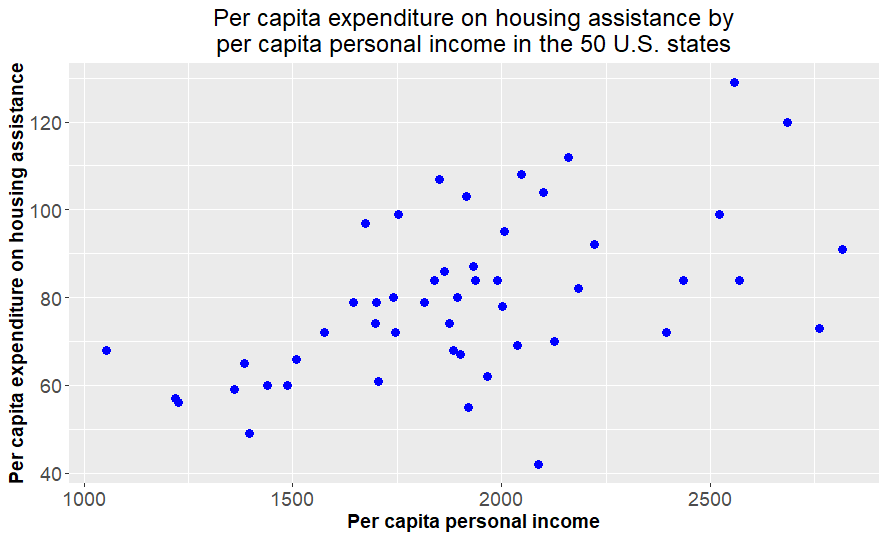
\includegraphics[width=0.9\linewidth]{Rplot1}
		\end{figure}
		
		In figure \ref{yx1}, data points scatter from the bottom-left corner of the graphic to the top-right corner. There seems to be some outliers both in the top and in the bottom of the graphic. Even so, the pattern suggests a positive linear relationship between $Y$ and $X1$.\\
		
		\newpage
		
		\textbf{2. Relationship between $Y$ and $X2$:}

		\vspace{.5cm}
		
		\lstinputlisting[language=R, firstline=94, lastline=102]{PS01_answersLucasDeMeloPrado.R}
		
		\begin{figure}[H]
			\centering
			\caption{}
			\label{yx2}
			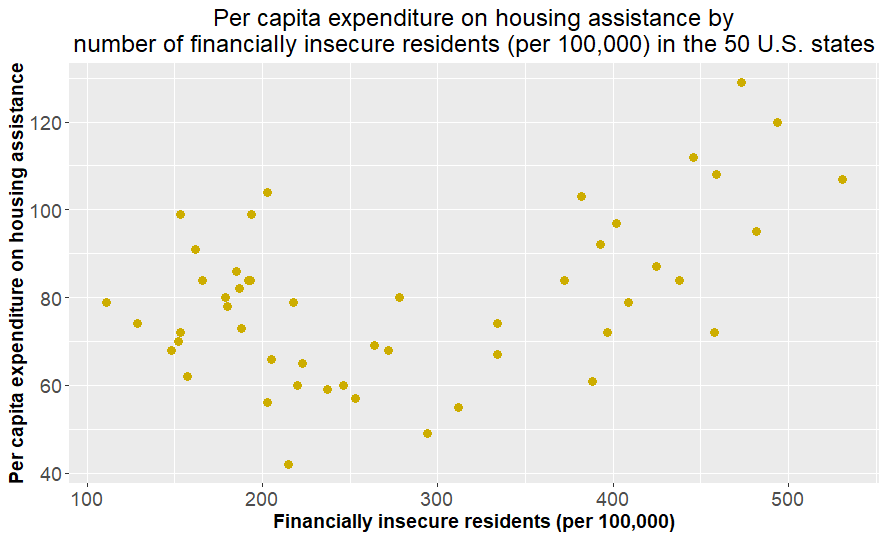
\includegraphics[width=0.9\linewidth]{Rplot2}
		\end{figure}
		
		Data points in figure \ref{yx2} are scattered in a U-shaped form, suggesting a non-linear relationship between $Y$ and $X2$.\\
		
		\newpage
		
		\textbf{3. Relationship between $Y$ and $X3$:}

		\vspace{.5cm}

		\lstinputlisting[language=R, firstline=104, lastline=112]{PS01_answersLucasDeMeloPrado.R}		
		
		\begin{figure}[H]
			\centering
			\caption{}
			\label{yx3}
			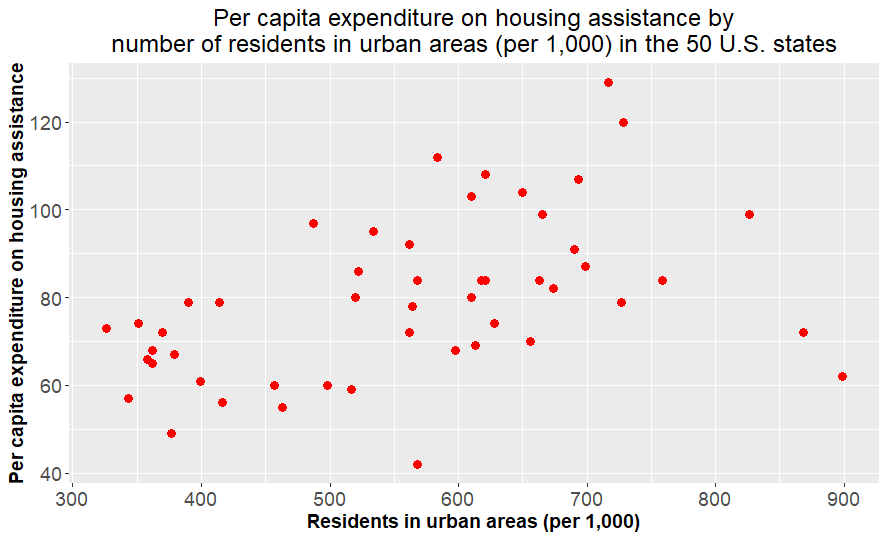
\includegraphics[width=0.9\linewidth]{Rplot3}
		\end{figure}
		
		In figure \ref{yx3}, most data concentrate in the bottom-left corner and the center of the graphic. The pattern suggests a positive linear relationship between $Y$ and $X3$.\\
		
		\newpage
		
		\textbf{4. Relationship between $X1$ and $X2$:}

		\vspace{.5cm}

		\lstinputlisting[language=R, firstline=114, lastline=122]{PS01_answersLucasDeMeloPrado.R}

		\begin{figure}[H]
			\centering
			\caption{}
			\label{x1x2}
			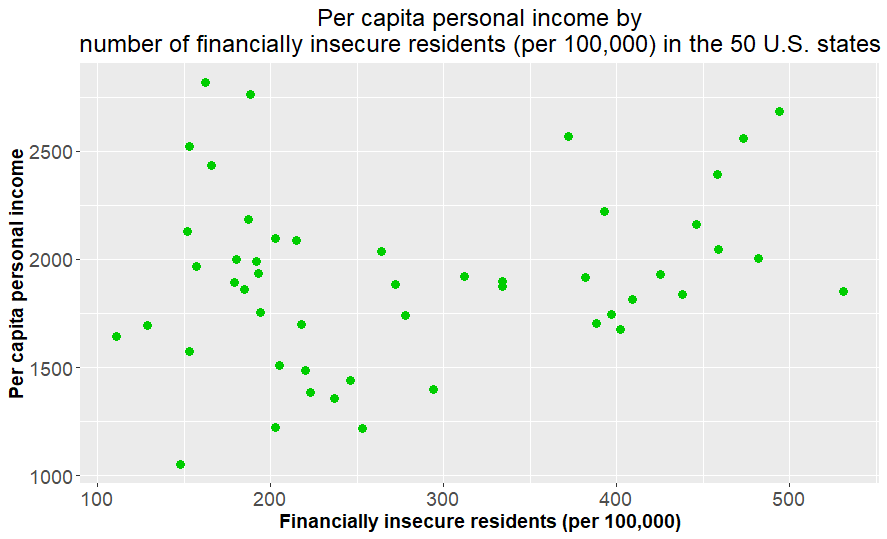
\includegraphics[width=0.9\linewidth]{Rplot4}
		\end{figure}
		
		Data points are scattered all over figure \ref{x1x2}, with no distinctive shape. The graphic does not allow any inference about the relationship between $X1$ and $X2$.\\
		
		\newpage
		
		\textbf{5. Relationship between $X1$ and $X3$:}

		\vspace{.5cm}		

		\lstinputlisting[language=R, firstline=124, lastline=132]{PS01_answersLucasDeMeloPrado.R}

		\begin{figure}[H]
			\centering
			\caption{}
			\label{x1x3}
			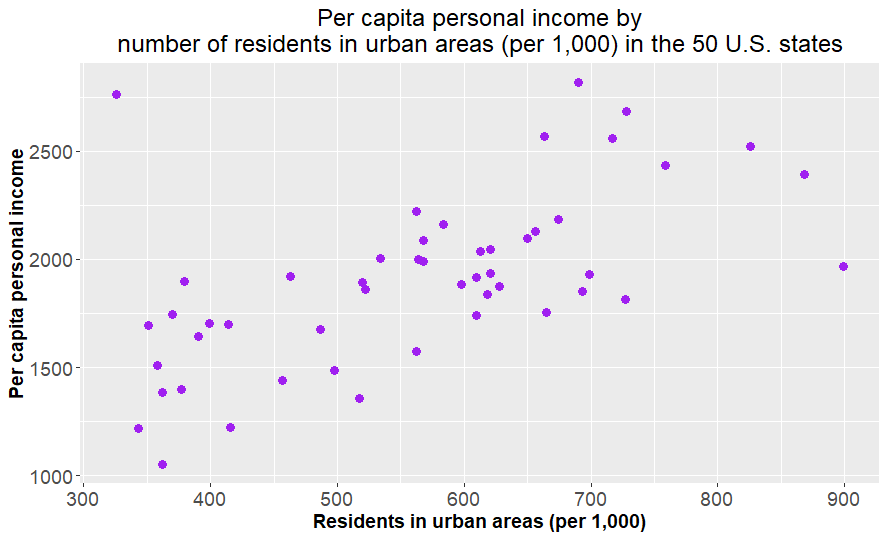
\includegraphics[width=0.9\linewidth]{Rplot5}
		\end{figure}
		
		Data in figure \ref{x1x3} scatter from the bottom-left corner of the graphic to the top-right one. Apart from the outlier in the top-left corner, the scatter pattern suggests a positive linear relationship between $X1$ and $X3$.\\
		
		\newpage
		
		\textbf{6. Relationship between $X2$ and $X3$:}

		\vspace{.5cm}

		\lstinputlisting[language=R, firstline=134, lastline=142]{PS01_answersLucasDeMeloPrado.R}

		\begin{figure}[H]
			\centering
			\caption{}
			\label{x2x3}
			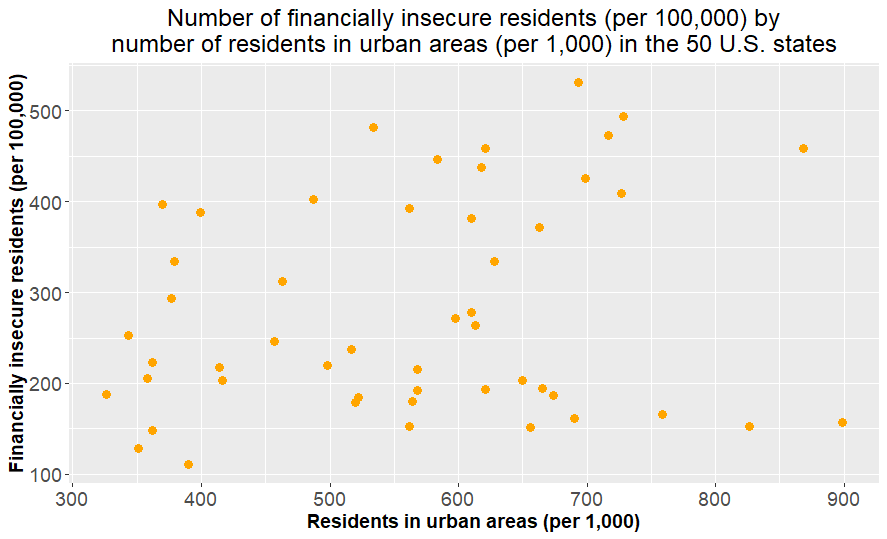
\includegraphics[width=0.9\linewidth]{Rplot6}
		\end{figure}
		
		Data are scattered all over figure \ref{x2x3}, with no distinctive shape. The graphic does not allow any inference about the relationship between $X2$ and $X3$.\\
		
		\newpage
		
		\item
		\textit{Please plot the relationship between \emph{Y} and \emph{Region}. On average, which region has the highest per capita expenditure on housing assistance?}

		\vspace{.5cm}

		\lstinputlisting[language=R, firstline=144, lastline=153]{PS01_answersLucasDeMeloPrado.R}

		\begin{figure}[H]
			\centering
			\caption{}
			\label{yRegion}
			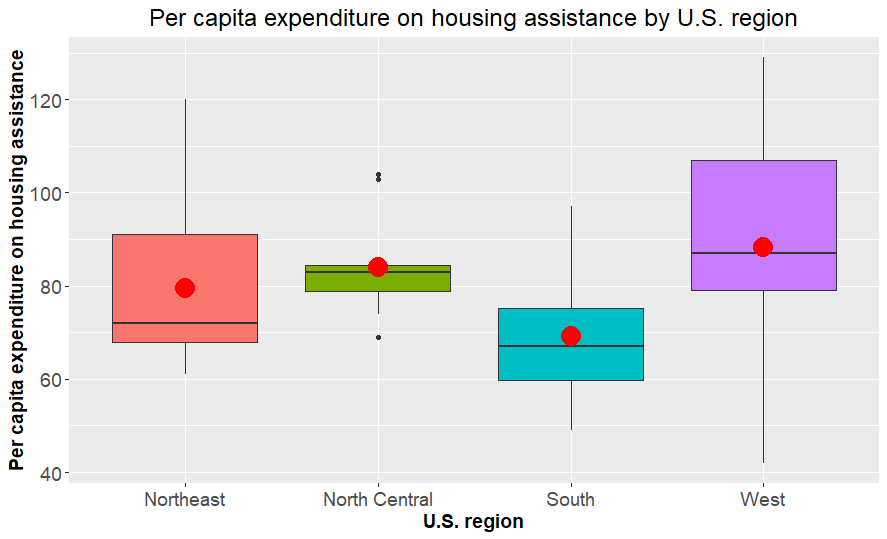
\includegraphics[width=0.9\linewidth]{Rplot7}
		\end{figure}
		
		The West presents the highest mean (red dots), the highest median (horizontal bars) and the highest interquartile interval (boxes) among the four regions. Therefore, by those three measures, data indicate that \textbf{the West has, on average, the highest \textit{per capita} expenditure on housing assistance}.
				
		\newpage
	
		\item
		\textit{Please plot the relationship between \emph{Y} and \emph{X1}. Describe this graph and the relationship. Reproduce the above graph including one more variable \emph{Region} and display different regions with different types of symbols and colors.}

		\vspace{.5cm}

		\lstinputlisting[language=R, firstline=155, lastline=163]{PS01_answersLucasDeMeloPrado.R}

		\begin{figure}[H]
			\centering
			\caption{}
			\label{yx1again}
			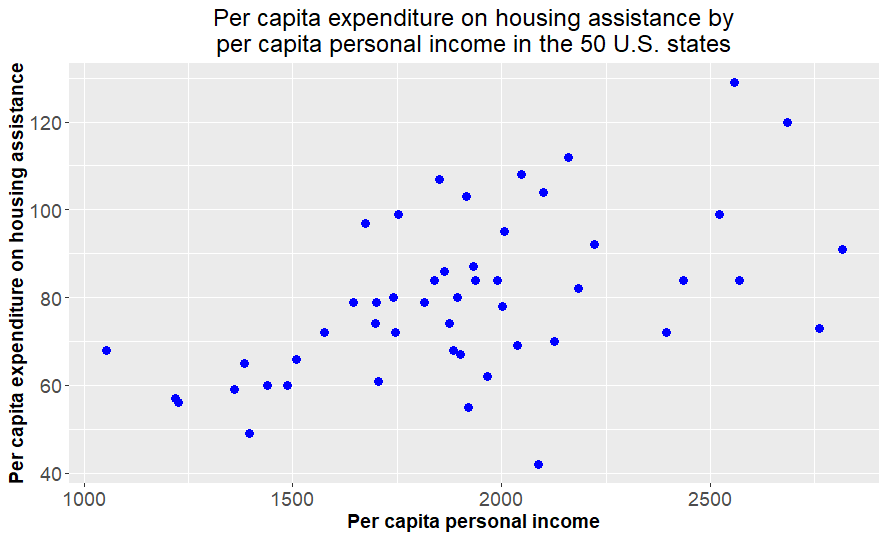
\includegraphics[width=0.9\linewidth]{Rplot8}
		\end{figure}
		
		In figure \ref{yx1again}, data points scatter from the bottom-left corner of the graphic to the top-right corner. There seems to be some outliers both in the top and in the bottom of the graphic. Even so, the pattern suggests a positive linear relationship between these two variables.\\
		
		Figure \ref{yx1Region} displays the same scatter plot, but different regions in the U.S. are represented as different types of symbols and colors.

		\vspace{.5cm}

		\lstinputlisting[language=R, firstline=165, lastline=176]{PS01_answersLucasDeMeloPrado.R}

		\begin{figure}[H]
			\centering
			\caption{}
			\label{yx1Region}
			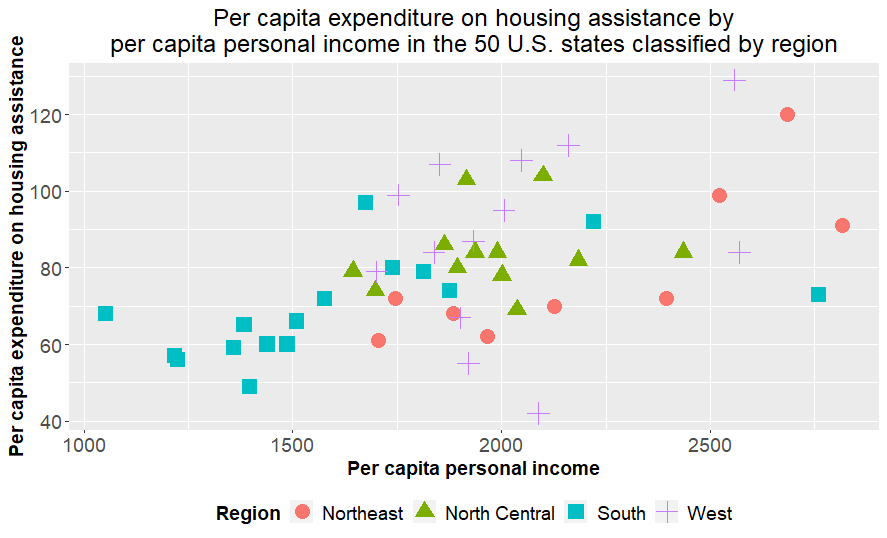
\includegraphics[width=0.9\linewidth]{Rplot9}
		\end{figure}
				
	\end{itemize}
		
\end{document}
